%Author Alex Clemmer
%CS 4150 Algorithms
%Assignment 04:
\documentclass[a4paper]{article}
\usepackage[pdftex]{graphicx}
\usepackage{fancyvrb}
\usepackage{multirow}
\usepackage{amssymb}
\usepackage{amsmath}
\usepackage{fullpage}
\addtolength{\oddsidemargin}{-.05in}
	\addtolength{\evensidemargin}{-.05in}
	\addtolength{\textwidth}{.25in}

	\addtolength{\textheight}{.25in}
\begin{document}

\section*{Assignment 04}
Alex Clemmer\\
Student number: u0458675

\section*{Hypothesis}

The assignments give us that adding elements into a static array is $O(k)$. This ``suggests" that the runtime for appending to a dynamic array would be ``the cost of doing 3k store operations" on some static array. We want to create and experiment to analyze this claim.

\section*{Procedure}

\subsubsection*{Foreward} One of the main weaknesses of my last assignment is that I did not have a systematic approach for creating the timing suite. This time, I did.

I started by just timing how long it took to allocate things to the array. Then I added code that spun the method for a few seconds before. Then I added code to time the loop itself, and subtract it from the total running time. At each point, I stopped and ran the program. If my code brought me closer to what I expected, I continued. If not, I fixed it.

The big insight here is that in my last assignment, I really just threw code onto the canvas. By incrementally developing the timing patterns, I was able to see in real time what did and did not work. This made my timing development both smoother and (probably) more correct.

\subsubsection*{How it works}

First, there were a couple of things that I found had no discernible effect on timing. First, it did not seem to matter whether I allocated one particular integer, or a lot of random integers. It also did not seem to matter, surprisingly enough, whether the integer was a variable or a literal.

One thing that did matter, a lot, was whether I used $\texttt{int}$ or $\texttt{Integer}$. I used the latter, but this may not have been the best choice. Either way, when I switched my static array from primitives to boxed primitives, the gap between their running time diminished from 9 times to ~2-3 times.

Whether we spun the allocation for a couple of seconds before actually running the experiment made our results much less erratic. In the case of the dynamic array, running add repeatedly caused the array to expand, so it was necessary to allocate a new $\texttt{ArrayList}$ just before the actual experiment. When I did not, the gap between the runtime of the dynamic array versus the static array was a $\textit{lot}$ smaller.

Another thing that was important for the dynamic array was to call the garbage collector. Oddly even though $\textit{not}$ calling the garbage collector did not actually cause a memory overflow error, it did make the results much less erratic.

The last, and most important thing, was size. Larger sizes were universally erratic and unpredictable. Smaller sizes were the only manageable data. I was informed of this by another student, and it seems that Joe said this in class.

\subsubsection*{Also important}

To actually time the operations, we stuck the actual allocation operation inside a loop. All the things listed before were important, but this was the actual testing mechanism. In order to do this, we just bookended the timing operations around the loop, and the timed the dry loop and subtracted that from the time.

\section*{Results}

The first graph below show both the time taken to execute one allocation operation as a function of the total number of operations executed. The second shows the total execution time of $x$ amount of operations. The data they are based on are below.

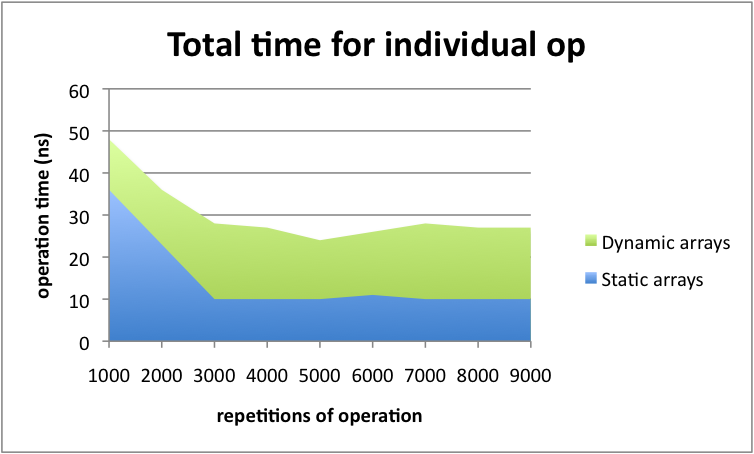
\includegraphics{avg_op_time.png}

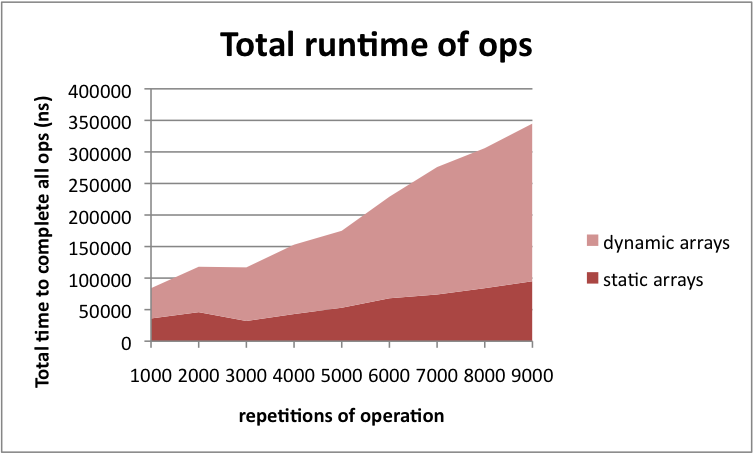
\includegraphics{total_runtime.png}

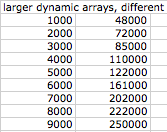
\includegraphics{dynarr_data.png}

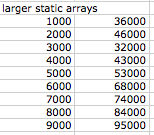
\includegraphics{statarr_data.png}

\section*{Analysis}

Strangely, the prediction is almost correct: the total coefficient is really almost right. The average for our dataset shows that the dynamic array takes about $\textbf{2.37}$ times more time per allocation operation than the static array. I bet for larger data sets this would even out to somewhere between 2.5 and 3.

The cleanliness of these results was really difficult to get, I should note. I took a lot of experimenting and smoothing, and I understand that while it is smooth, I assure you it is authentic. You said not to include the file, so I won't, but if you question the veracity of my claims, I will happily provide the java file.

\end{document}